\subsection{Analyse de santé du code}
L'analyse de la santé du code a été réalisée via l'outil \textbf{CodeScene} sur la période du 5 mai 2025 au 8 août 2025. 
Le projet \textbf{PuckLab} totalise 21\,250 lignes de code réparties sur 120 fichiers, pour un seul développeur actif et 44 commits effectués durant la période de développement.

Aucun risque actif n’a été identifié (voir la \autoref{fig:codescene_distribution}) et la tendance globale est stable, avec des scores de santé du code très élevés (voir la \autoref{fig:codescene_scores}).
Le \autoref{tab:codescene_thresholds} disponible en \autoref{sec:codescene} donne les interprétations des scores de santé de CodeScene.

\begin{figure}[H]
  \centering

  \begin{subfigure}[b]{0.48\linewidth}
    \centering
    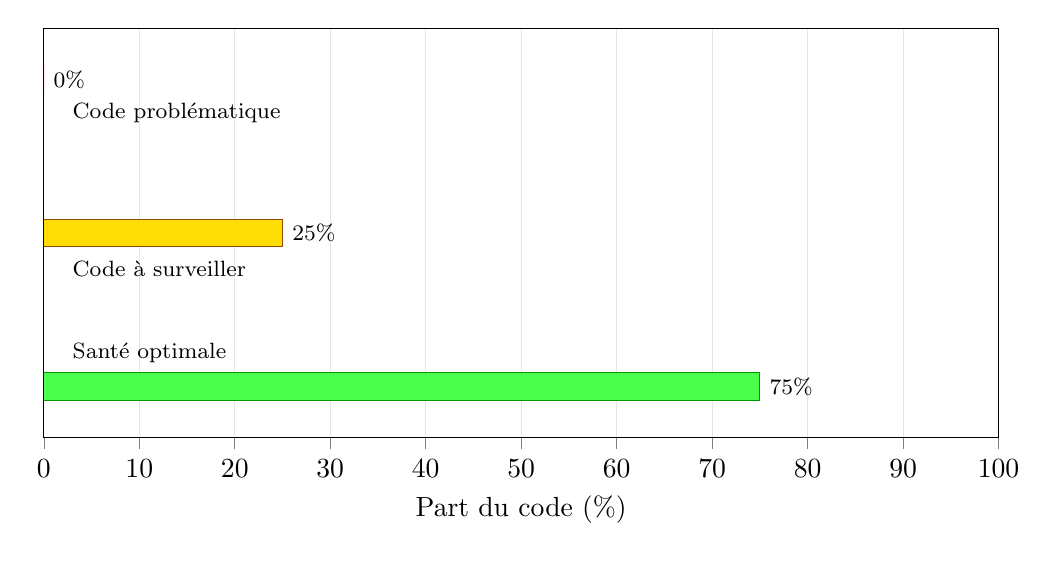
\begin{tikzpicture}
      \begin{axis}[
        xbar,
        scale only axis=true,
        trim axis left,
        xmin=0, xmax=100,
        width=\linewidth, height=5.2cm,
        bar width=10pt,
        ytick=\empty,
        xlabel={Part du code (\%)},
        nodes near coords={\pgfmathprintnumber\pgfplotspointmeta\%},
        every node near coord/.append style={
          font=\footnotesize, text=black,
          /pgf/number format/.cd,fixed,precision=0
        },
        nodes near coords align={horizontal},
        point meta=rawx,
        grid=both,
        grid style={gray!20},
        y dir=reverse,
        enlarge y limits=0.35,
        tick align=outside,
        tick pos=left,
      ]
        \addplot+[fill=green!70, draw=green!60!black]  coordinates {(75,3)};
        \addplot+[fill=yellow!80!orange, draw=orange!60!black] coordinates {(25,2)};
        \addplot+[fill=red!70,   draw=red!60!black]   coordinates {(0,1)};

        \node[anchor=west, font=\footnotesize] at (axis cs:2,3) {Santé optimale};
        \node[anchor=west, font=\footnotesize] at (axis cs:2,2.3) {Code à surveiller};
        \node[anchor=west, font=\footnotesize] at (axis cs:2,1) {Code problématique};
      \end{axis}
    \end{tikzpicture}
    \subcaption{Répartition de la santé du code}
    \label{fig:codescene_distribution}
  \end{subfigure}
  \hfill
  \begin{subfigure}[b]{0.48\linewidth}
    \centering
    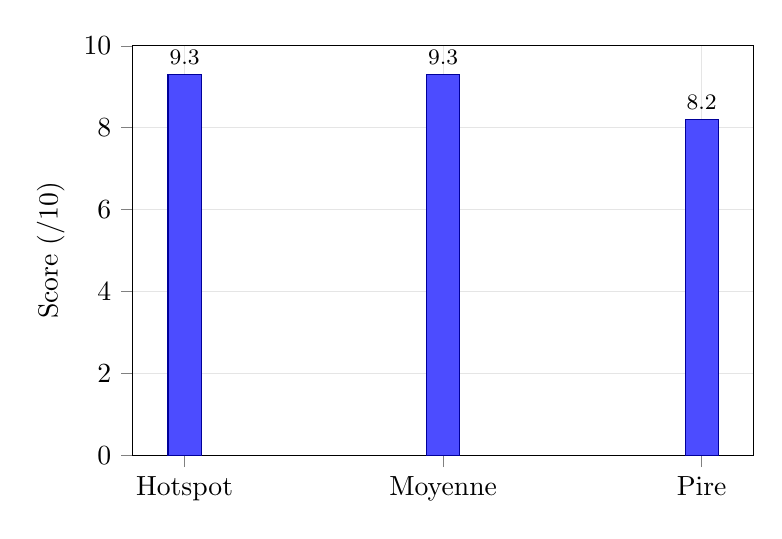
\begin{tikzpicture}
      \begin{axis}[
        ybar,
        scale only axis=true,
        ymin=0, ymax=10,
        width=0.65\linewidth, height=5.2cm,
        bar width=12pt,
        symbolic x coords={Hotspot, Moyenne, Pire},
        xtick=data,
        ylabel={Score (/10)},
        nodes near coords,
        every node near coord/.append style={font=\footnotesize, text=black},
        nodes near coords align={vertical},
        tick align=outside,
        tick pos=left,
        grid=both,
        grid style={gray!20},
        ymajorgrids=true
      ]
        \addplot[fill=blue!70, draw=blue!60!black] coordinates {
          (Hotspot, 9.3)
          (Moyenne, 9.3)
          (Pire, 8.2)
        };
      \end{axis}
    \end{tikzpicture}
    \subcaption{Scores Code Health}
    \label{fig:codescene_scores}
  \end{subfigure}

  \caption{Synthèse CodeScene : répartition et scores}
  \label{fig:codescene_side_by_side}
\end{figure}

\paragraph{Analyse synthétique}
Ces résultats indiquent un projet \textbf{hautement maintenable}, avec :
\begin{itemize}
    \item 75\% du code classé sain et aucun segment en zone rouge ;
    \item des scores homogènes autour de 9/10, y compris pour le pire fichier ;
    \item une stabilité sur la période sans dégradation de la qualité.
\end{itemize}

La métrique \textit{"pire composant"} correspond au score de santé le plus bas relevé dans l’ensemble du code.
Dans le cas présent, ce score est de \textbf{8,2/10}, ce qui reste largement dans la plage considérée comme \textit{saine} par CodeScene (7 à 10).
Il est resté stable sur toute la période de développement, sans signe de dégradation.
De plus, la base de code ne contient aucune portion marquée comme \textit{non saine} (rouge) et aucun risque actif identifié.
Ainsi, même le composant le moins bien noté présente un niveau de qualité et de maintenabilité élevé, illustrant la solidité globale de l’architecture et des pratiques mises en œuvre.